A point of presence (PoP) is an artificial demarcation point or interface point between communicating entities.
In our case we are refering to optical fibre interconnection points.
From 2010 until now the guifi.net community has raised six points of presence over the Catalan territory.
This POPs are following the network model of freedom and neutrality specified in the XOLN\ref{XOLN} licence.
Thus anyone is able to connect to them but always respecting the same conditions.
From a general perspective guifi.net community is building a set of neutral exchange points, leaving the
infraestructure available to the individuals, associations or either companies.
\medskip
Figure \ref{fig:fibre_map} shows the fibre network map of guifi.net POPs (not all of them).

\bigskip

The current guifi.net POPs are managed, maintained and also economically sustained for the community. 
To interconnect all of them it is need to use third party infrastructure. The FFTH projects are able to deploy some kilometers
of optical fibre but not hundreds or even thousands.
\newline
In Catalonia there exist a set of deployed fibres which are owned by the Catalan goverment, available to any entity and 
rented for a regularized price. Most of the guifi.net POPs are connected to such network to interchange data
between them. Figure \ref{fig:xoc_map} shows a slice of the network fibre map provided by the goberment. 

\begin{figure}[htbp]
  \centering
  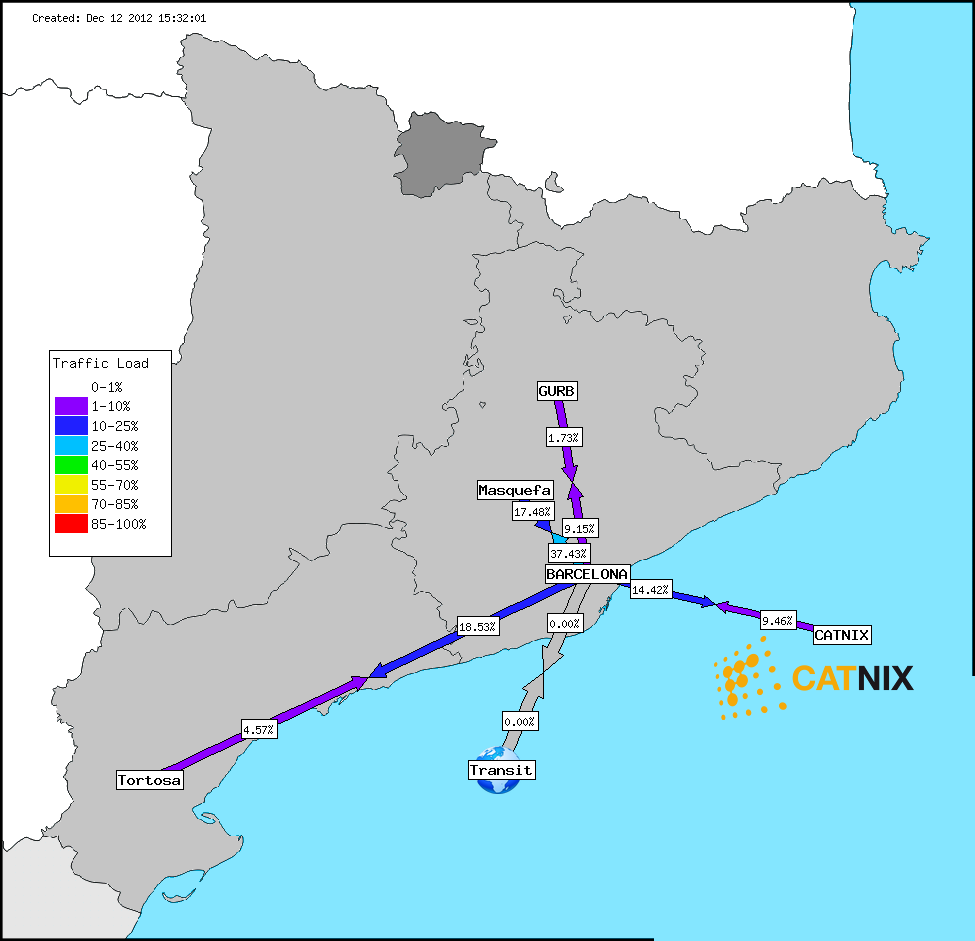
\includegraphics[scale=.35]{sect3/figures/pops_network_map.eps} 
%% use convert command to convert formats "convert pops_network_map.png pops_network_map.eps" e.g. 
  \caption{Guifi.net fibre POPs network map}
  \label{fig:fibre_map}
\end{figure}

\begin{figure}[htbp]
  \centering
  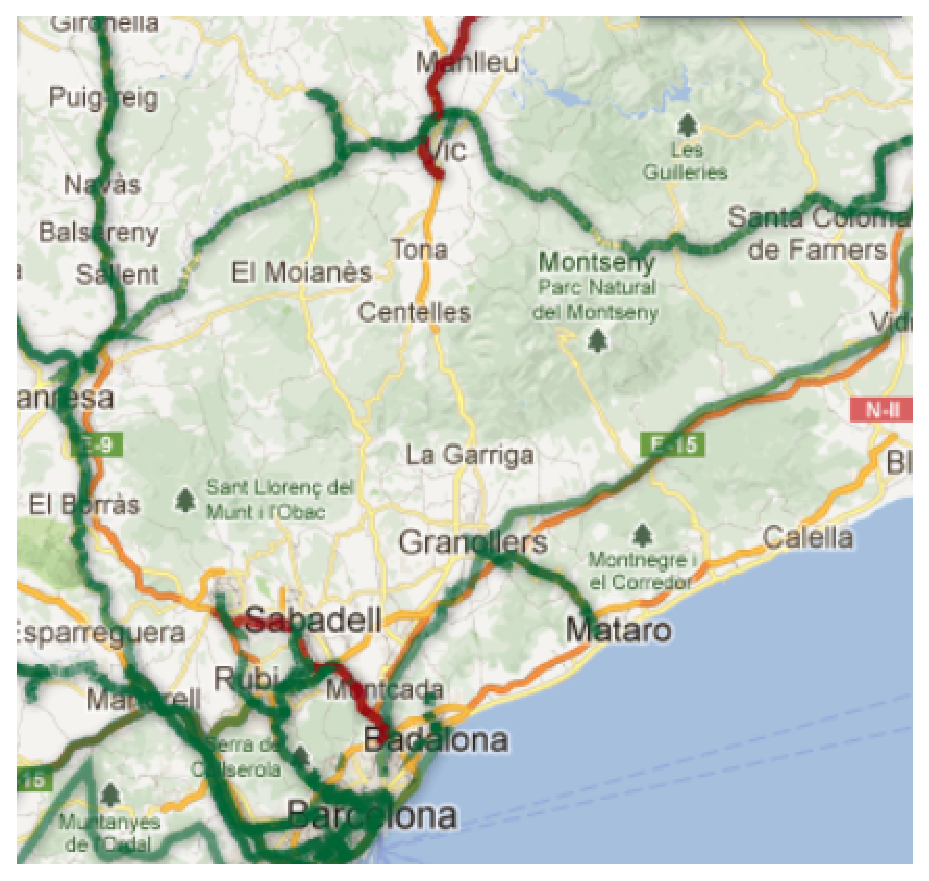
\includegraphics[scale=.5]{sect3/figures/xoc_map.eps} 
  \caption{Available regularized fibre}
  \label{fig:xoc_map}
\end{figure}



\subsection{Pilot's deployments}

\subsubsection{Gurb}
\begin{figure}[htbp]
  \centering
  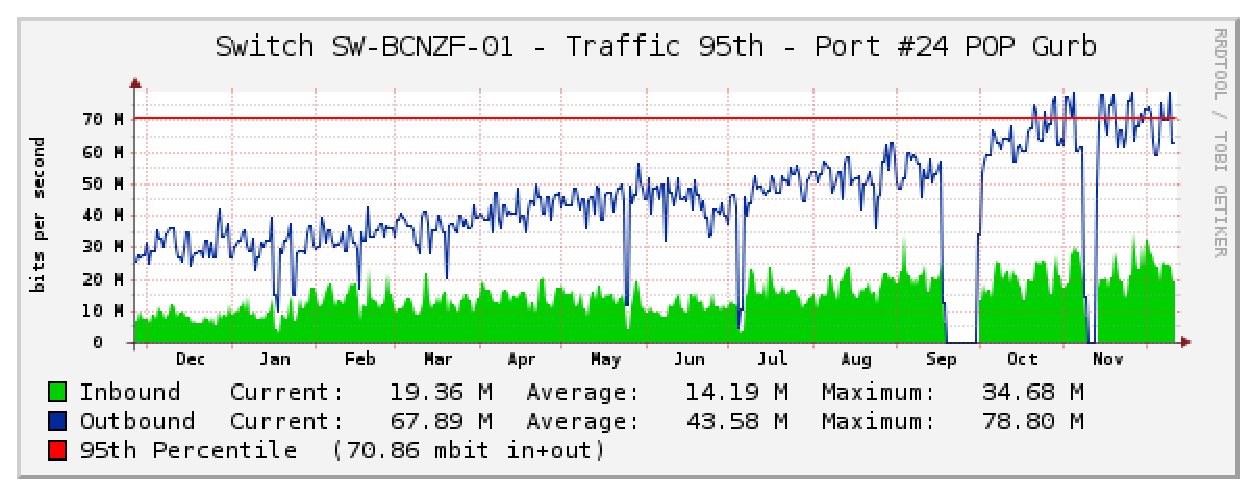
\includegraphics[scale=.65]{sect3/figures/gurb_network_load_year.eps} 
  \caption{Gurb's POP network load (year)}
  \label{fig:gurb_net_load}
\end{figure}


\subsubsection{Vic}

\begin{figure}[htbp]
  \centering
  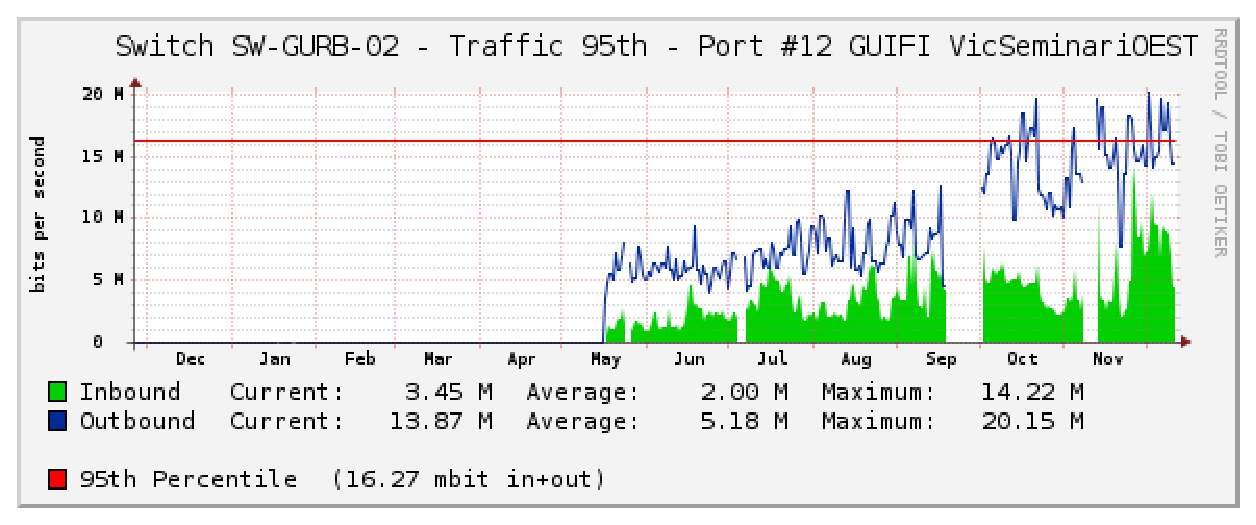
\includegraphics[scale=.65]{sect3/figures/vic_network_load_year.eps} 
  \caption{Vic's POP network load (year)}
  \label{fig:vic_net_load}
\end{figure}



\subsection{Other deployments}

\subsubsection{CATNIX-TELVENT}

\bigskip 

CATNIX\footnote{\url{http://www.catnix.net}} is the name of the internet exchange point (IX) of Catalonia. 
It is a physical infrastructure provided by the goberment to leave the network operators exchange their 
information and connect their networks (autonomous systems). 

\medskip
All guifi.net POPs terminate to such infrastructure (as can be shown in figure \ref{fig:fibre_map}) where
all of them connect together to became part of the main community network. 

\medskip
Guifi.net Foundation operates it's own backbone infrastructure using the ASN 49835 (Autonomous System Number). 
An open peering policy is followed to establish peering sessions with all potential partners.
The Foundation is part of the CATNIX, so it is also possible to exchange data with other ISP and
rent Internet uplink directly to an international carrier. Right now there is one symetric Internet gigabit 
available. 
\newline
This is probably the most important POP of the current guifi.net network infraestructure.


\begin{figure}[htbp]
  \centering
  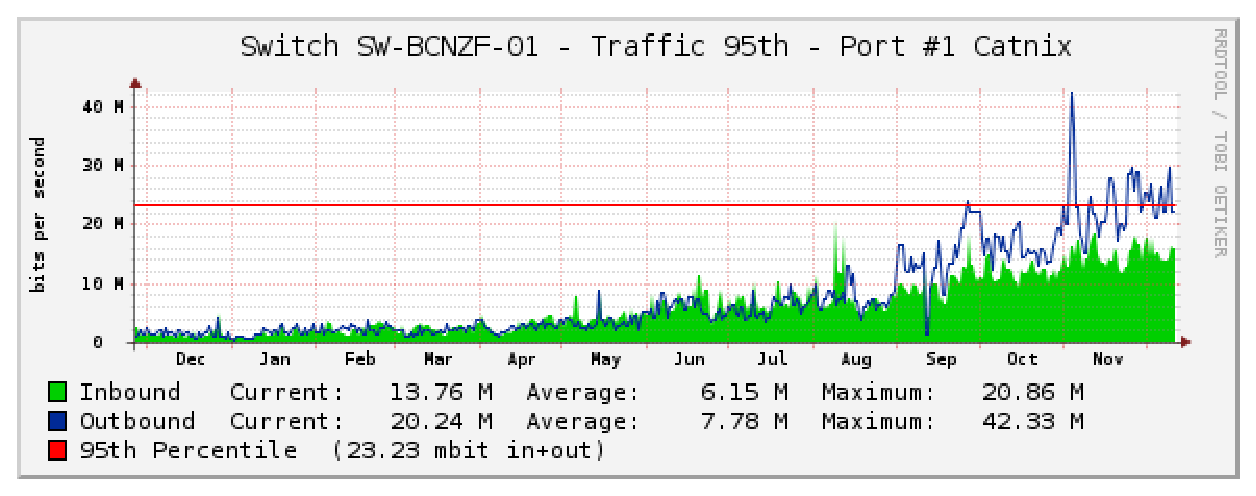
\includegraphics[scale=.65]{sect3/figures/catnix_network_load_year.eps} 
  \caption{CATNIX's POP network load (year)}
  \label{fig:vic_net_load}
\end{figure}


